\section{Case Study: Shopping Cart}
\label{sec:case}
In this section, we develop two different designs for a distributed
shopping-cart service in Bloom.\footnote{The complete source code for both
  implementations can be found at
  \smallurl{https://trac.declarativity.net/browser/bud/test/cart}.}  In a
shopping cart system, clients add and remove items from their shopping cart. To
provide fault tolerance and persistence, the content of the cart is stored by a
collection of server replicas. Once a client has finished shopping, they perform
a ``checkout'' request, which returns the final state of their cart.

After presenting the abstract shopping cart protocol and a simple client
program, we implement a ``destructive,'' state-modifying shopping cart service
that uses the key-value store we developed in the Section~\ref{sec:kvs}. Second,
we illustrate a ``disorderly'' cart that accumulates updates in a set-wise
fashion, summarizing updates at checkout into a final result.  These two
different designs illustrate our analysis tools and the way they inform design
decisions for distributed programming.

\subsection{Shopping Cart Client}

An abstract shopping cart protocol is presented in
Figure~\ref{fig:cart-protocol}. Figure~\ref{fig:cart-client} contains a simple
shopping cart client program: it takes client operations (represented as
\texttt{client\_action} and \texttt{client\_checkout} facts) and sends them to
the shopping cart service using the CartProtocol. We assume that clients have
some mechanism for choosing which cart server replica to send requests to (e.g.,
based on load balancing).

\begin{figure}[t]
\begin{scriptsize}
\begin{lstlisting}
module CartProtocol
  def state
    channel :action_msg, (*\label{line:dec_chan_beg}*)
      ['@server', 'client', 'session', 'reqid'],
      ['item', 'action'] (*\label{line:dec_chan_end}*)
    channel :checkout_msg,
      ['@server', 'client', 'session', 'reqid']
    channel :response_msg,
      ['@client', 'server', 'session', 'item'], ['cnt']
  end
end

module CartClientProtocol
  def state
    interface input, :client_action, (*\label{line:dec_in_interface}*)
      ['server', 'session', 'reqid'], ['item', 'action'] 
    interface input, :client_checkout,
      ['server', 'session', 'reqid']
    interface output, :client_response, 
      ['client', 'server', 'session'], ['item', 'cnt']
  end
end
\end{lstlisting}
\vspace{-10pt}
\caption{Abstract shopping cart protocol.}
\label{fig:cart-protocol}
\end{scriptsize}
\vspace{-2pt}
\end{figure}

\begin{figure}[t]
\begin{scriptsize}
\begin{lstlisting}
module CartClient
  include CartProtocol
  include CartClientProtocol

  declare
  def client
    action_msg <~ client_action.map do |a| 
      [a.server, @addy, a.session, a.reqid, a.item, a.action] (*\label{line:des_client_action}*)
    end
    checkout_msg <~ client_checkout.map do |a| 
      [a.server, @addy, a.session, a.reqid]
    end
    client_response <= response_msg
  end
end
\end{lstlisting}
\vspace{-10pt}
\caption{Shopping cart client implementation.}
\label{fig:cart-client}
\end{scriptsize}
\vspace{-2pt}
\end{figure}

\subsection{``Destructive'' Shopping Cart Service}

\begin{figure}[t]
\begin{scriptsize}
\begin{lstlisting}
module DestructiveCart
  include CartProtocol
  include KVSProtocol

  declare (*\label{line:des_declare}*)
  def do_action
    kvget <= action_msg.map{|a| [a.reqid, a.key]}

    kvput <= action_msg.map do |a|
      if a.action == "A" (*\label{line:des_kvstate_gen_beg}*)
        unless kvget_response.map{|b| b.key}.include? a.session (*\label{line:des_kvstate_check}*)
          [a.server, a.client, a.session, a.reqid, [a.item]]
        end
      end (*\label{line:des_kvstate_gen_end}*)
    end

    old_state = join [kvget_response, action_msg],
                     [kvget_response.key, action_msg.session]  (*\label{line:des_join_kvstate_action_msg}*)
    kvput <= old_state.map do |b, a|
      if a.action == "A" (*\label{line:des_replace_beg}*)
        [a.server, a.client, a.session, 
         a.reqid, b.value.push(a.item)]
      elsif a.action == "D"
        [a.server, a.client, a.session, 
         a.reqid, delete_one(b.value, a.item)]
      end (*\label{line:des_replace_end}*)
    end
  end

  declare
  def do_checkout
    kvget <= checkout_msg.map{|c| [c.reqid, c.session]} (*\label{line:kvget-beg}*)
    lookup = join [kvget_response, checkout_msg],
                  [kvget_response.key, checkout_msg.session]
    response_msg <~ lookup.map do |r, c|
      [c.client, c.server, c.session, r.key, r.value] (*\label{line:kvget-end}*)
    end
  end
end
\end{lstlisting}
\vspace{-10pt}
\caption{Destructive cart implementation.}
\label{fig:dest-cart}
\end{scriptsize}
\vspace{-2pt}
\end{figure}

We begin with a shopping cart service built on a key-value store.  Each cart is
a \texttt{(key,value)} pair, where \texttt{key} is a unique session identifier
and \texttt{value} is an object containing the session's state, including a Ruby
array that holds the items currently in the cart. Adding or deleting items from
the cart result in ``destructive'' updates: the value associated with the key is
replaced by a new value that reflects the effect of the update. Deletion
requests are ignored if the item they refer to does not exist in the cart.

Figure~\ref{fig:dest-cart} shows the Bloom code for this design. The
\texttt{kvput} collection is provided by the abstract KVSProtocol described in
Section~\ref{sec:kvs}. Our shopping cart service would work with any concrete
realization of the KVSProtocol; we will choose to use the replicated key-value
store (Section~\ref{sec:rep-kvs}) to provide fault-tolerance.

When client actions arrive from the CartClient, the cart service checks to see
if there is a record in the key-value store associated with the client's
session. If no record is found (i.e., this is the first operation for a new
session), then
lines~\ref{line:des_kvstate_gen_beg}--\ref{line:des_kvstate_gen_end} generate an
entry for the new session in \texttt{kvstate}.  Otherwise, the join conditions
in line~\ref{line:des_join_kvstate_action_msg} are satisfied and
lines~\ref{line:des_replace_beg}--\ref{line:des_replace_end} ``replace'' the
value in the key-value store with an updated set of items for this session; this
uses the built-in overwriting capability provided by the key-value store.  When
a \texttt{checkout\_msg} appears at a server replica, the key-value store is
queried to retrieve the cart state associated with the given session
(lines~\ref{line:kvget-beg}--\ref{line:kvget-end}), and the results are returned
to the client.

\subsection{``Disorderly'' Shopping Cart Service}

\begin{figure}[t]
\begin{scriptsize}
\begin{lstlisting}
module DisorderlyCart
  include CartProtocol

  def state
    table :cart_action, ['session', 'item', 'action', 'reqid']
    table :action_cnt, ['session', 'item', 'action'], ['cnt']
    scratch :status, ['server', 'client', 'session', 'item'],
                     ['cnt']
  end

  declare
  def do_action
    cart_action <= action_msg.map do |c| (*\label{line:dis_action_msg_beg}*)
      [c.session, c.item, c.action, c.reqid] 
    end (*\label{line:dis_action_msg_end}*)
    action_cnt <= cart_action.group(  (*\label{line:dis_count_reqid_beg}*)
      [cart_action.session, cart_action.item, cart_action.action],
      count(cart_action.reqid))  (*\label{line:dis_count_reqid_end}*)
  end

  declare
  def do_checkout
    del_items = action_cnt.map{|a| a.item if a.action == "Del"} (*\label{line:dis_checkout_no_item_beg}*)
    status <= join([action_cnt, checkout_msg]).map do |a, c|
      if a.action == "Add" and not del_items.include? a.item
        [c.client, c.server, a.session, a.item, a.cnt] (*\label{line:dis_status_add}*)
      end
    end (*\label{line:dis_checkout_no_item_end}*)

    status <= join([action_cnt, action_cnt, (*\label{line:dis_checkout_item_beg}*)
                    checkout_msg]).map do |a1, a2, c|
      if a1.session == a2.session and a1.item == a2.item and
         a1.session == c.session and
         a1.action == "A" and a2.action == "D"
        [c.client, c.server, c.session, a1.item, a1.cnt - a2.cnt] (*\label{line:dis_status_diff}*)
      end
    end (*\label{line:dis_checkout_item_end}*)

    response_msg <~ status (*\label{line:dis_checkout_response}*)
  end
end
\end{lstlisting}
\vspace{-10pt}
\caption{Disorderly cart implementation.}
\label{fig:dis-cart}
\end{scriptsize}
\vspace{-2pt}
\end{figure}

Figure~\ref{fig:dis-cart} shows an alternative shopping cart implementation, in
which updates are monotonically accumulated in a set, and summed up only at
checkout.  Lines~\ref{line:dis_action_msg_beg}--\ref{line:dis_action_msg_end}
insert client updates into the persistent table \texttt{cart\_action}.
Lines~\ref{line:dis_count_reqid_beg}--\ref{line:dis_count_reqid_end} define
\texttt{action\_cnt} as an aggregate over \texttt{cart\_action}, in the style of
an SQL \texttt{GROUP BY} statement: for each item associated with a cart, we
separately count the number of times it was added and the number of times it was
deleted.
%Lines 5--16 define the collection \texttt{status} as the union of the session,
%item and action fields resulting from a 3-way join between the
%\texttt{checkout} message and two copies of \texttt{action\_cnt}---one
%corresponding to additions and one to deletions -- and the set of
%\texttt{action\_cnt}  tuples corresponding to items for which there is no
%deletion in a given session.
Lines~\ref{line:dis_checkout_no_item_beg}--\ref{line:dis_checkout_no_item_end}
ensure that when a \texttt{checkout\_msg} tuple arrives, \texttt{status}
contains a record for every added item for which there was no corresponding
deletion in the session.
Lines~\ref{line:dis_checkout_item_beg}--\ref{line:dis_checkout_item_end}
additionally define \texttt{status} as the 3-way join of the
\texttt{checkout\_msg} message and two copies of \texttt{action\_cnt}---one
corresponding to additions and one to deletions.  Thus, for each item,
\texttt{status} contains its final quantity: the difference between the number
of additions and deletions (line~\ref{line:dis_status_diff}), or simply the
number of additions if there are no deletions (line~\ref{line:dis_status_add}).
Upon the appearance of a \texttt{checkout\_msg}, the replica returns a
\texttt{response\_msg} to the client containing the final quantity
(line~\ref{line:dis_checkout_response}).

%Because the disorderly implementation does not use a separate storage system,
%it includes its own logic for state replication
%(lines~\ref{line:dis_join_action_msg_member}--\ref{line:dis_rep_end}).
%Line~\ref{line:dis_multicast} ensures that only the replica contacted by the
%client performs a multicast, by probing the table \texttt{member} to
%see if the \texttt{action\_msg} originated inside the quorum.

\subsection{Analysis}

\begin{figure}[t]
\centering
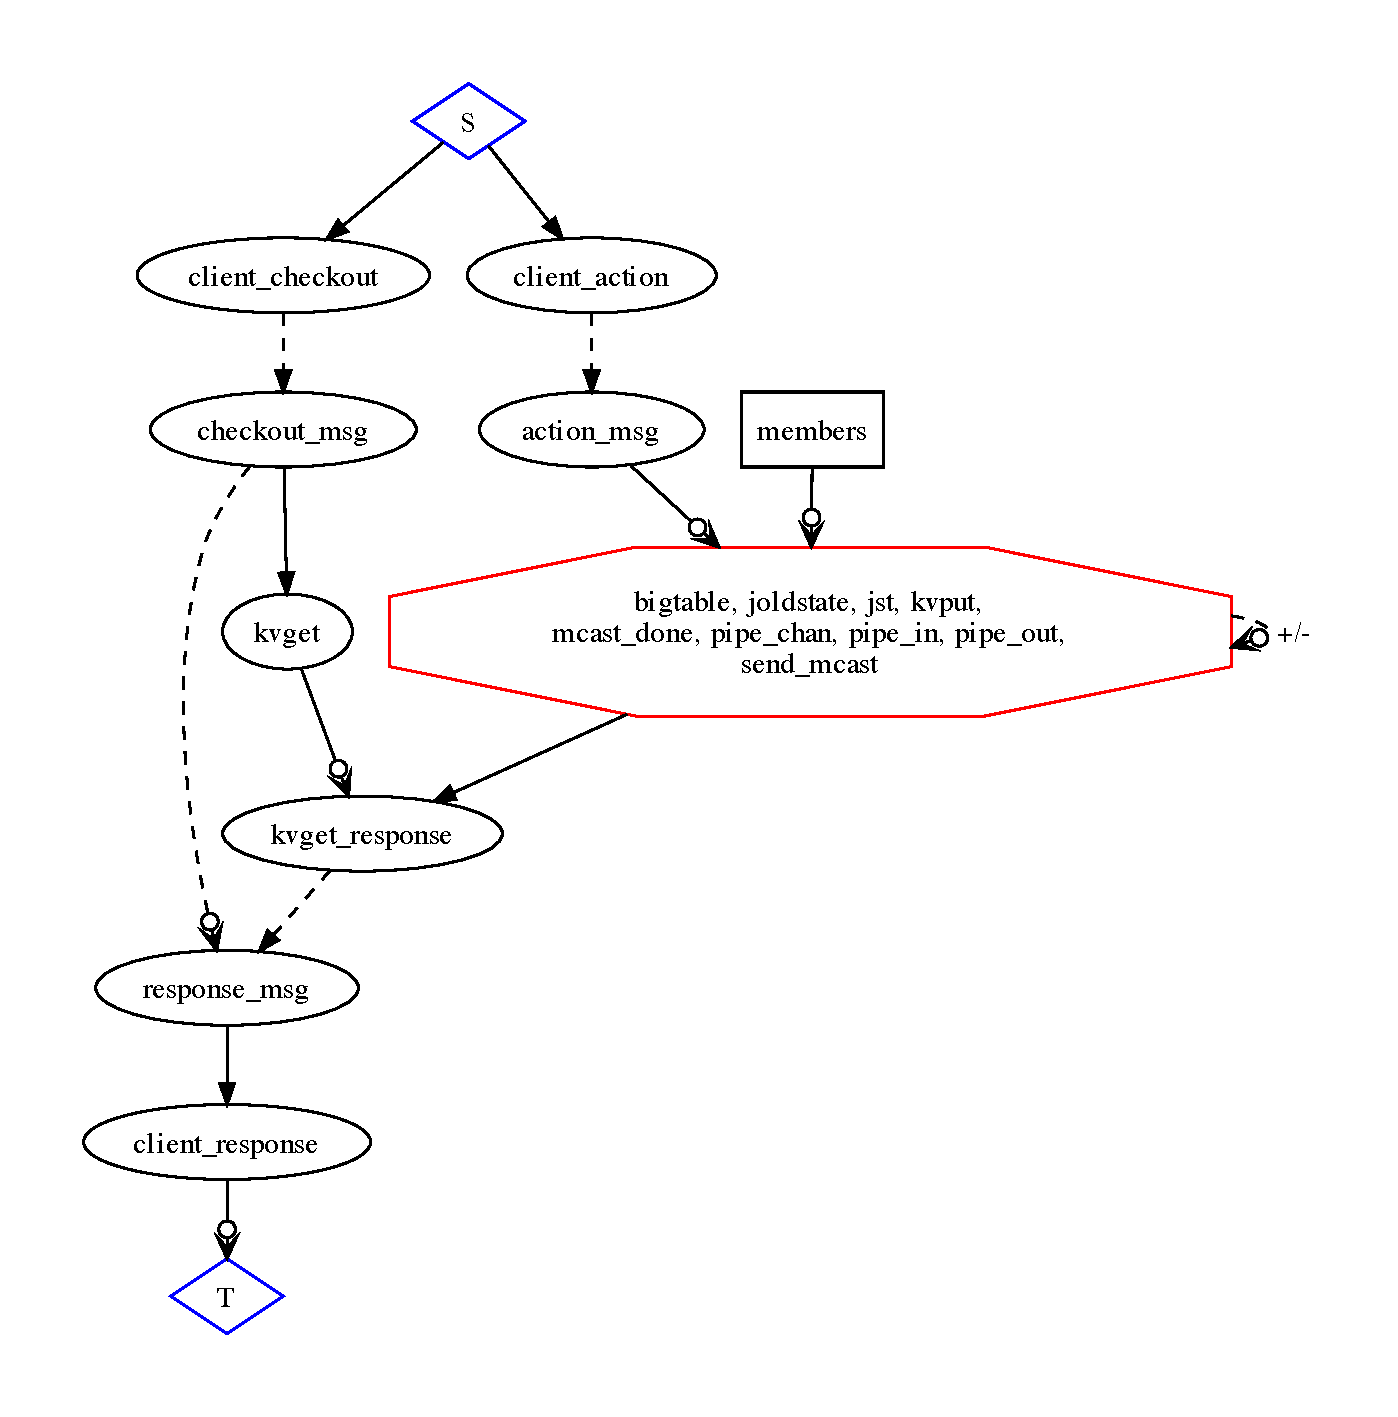
\includegraphics[width=1.1\linewidth]{fig/destructive_kvs.pdf}
\vspace{-10pt}
\caption{Visualization of the ``destructive'' cart program.  \jmh{These figs are a bit too small -- when I print them they're illegible.}}
\label{fig:pdg-destructive-kvs-analysis}
\vspace{-2pt}
\end{figure}

\begin{figure}[t]
\centering
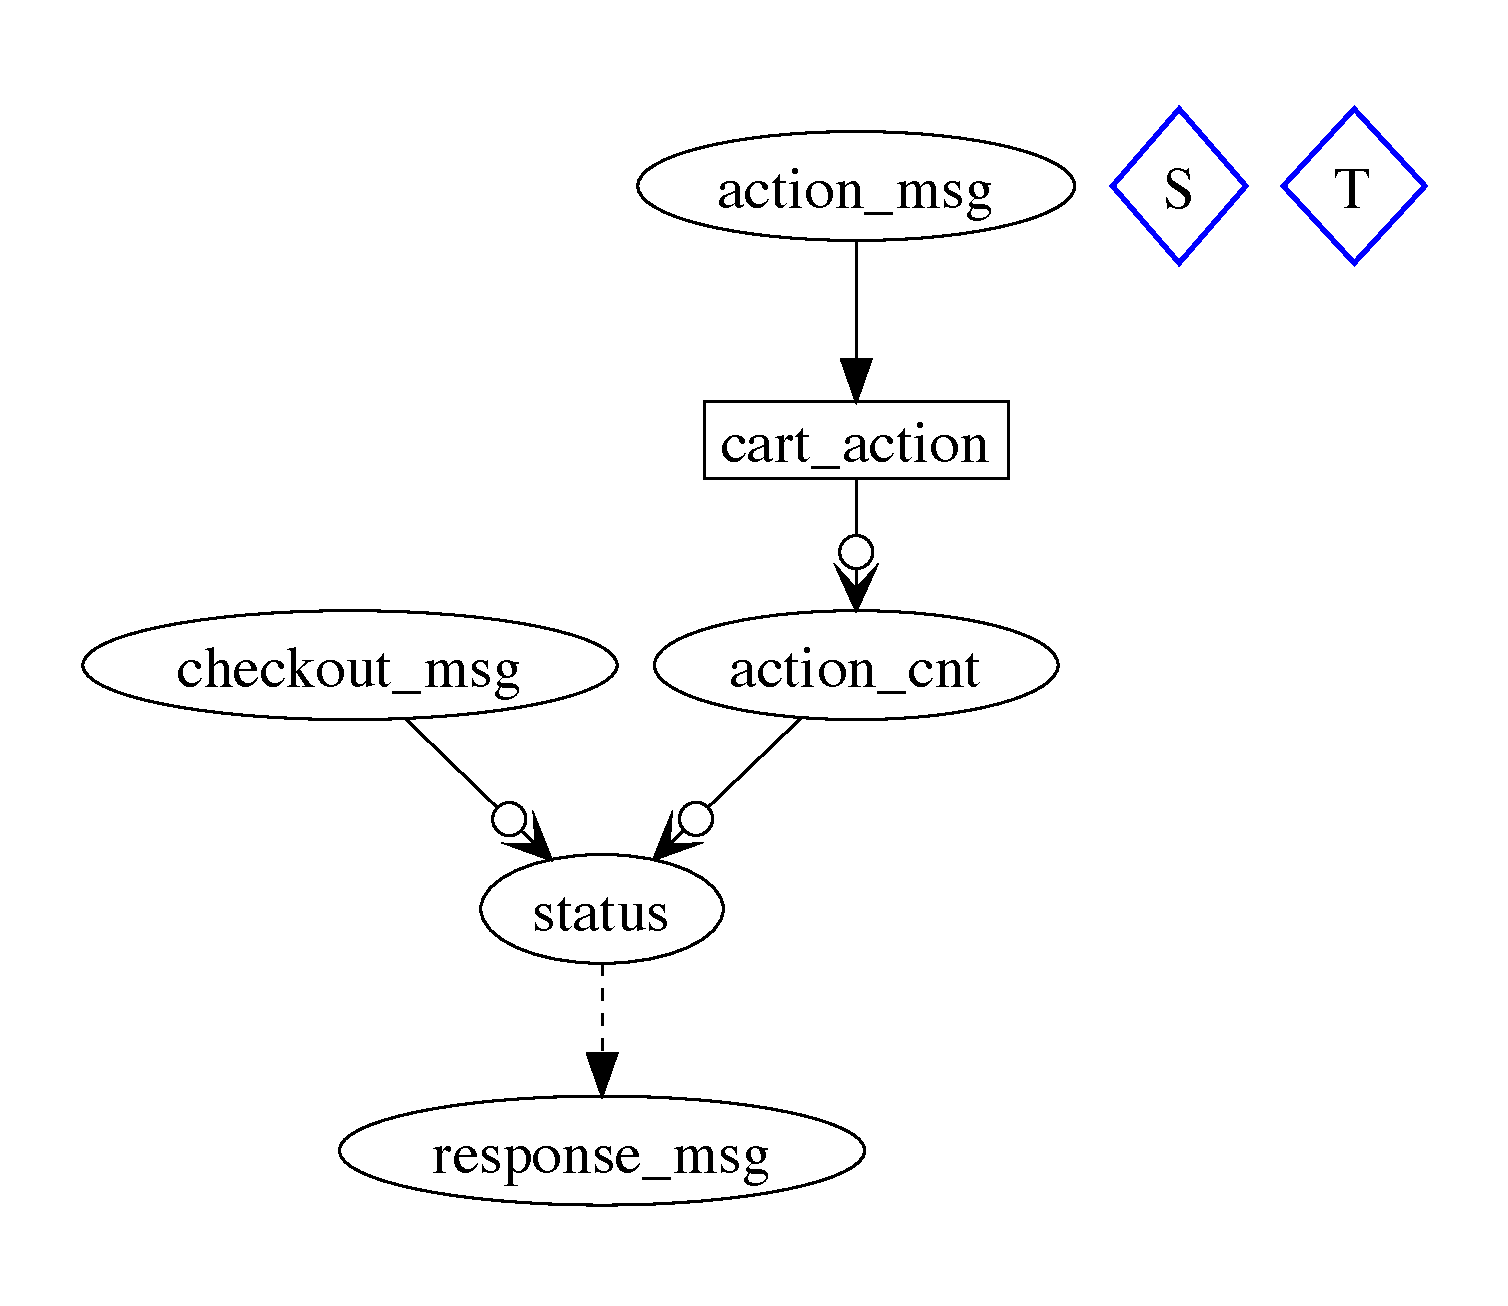
\includegraphics[width=0.8\linewidth]{fig/disorderly_base.pdf}
\vspace{-10pt}
\caption{Visualization of the basic ``disorderly'' cart program.}
\label{fig:pdg-disorderly-base}
\vspace{-2pt}
\end{figure}

\begin{figure}[t]
\centering
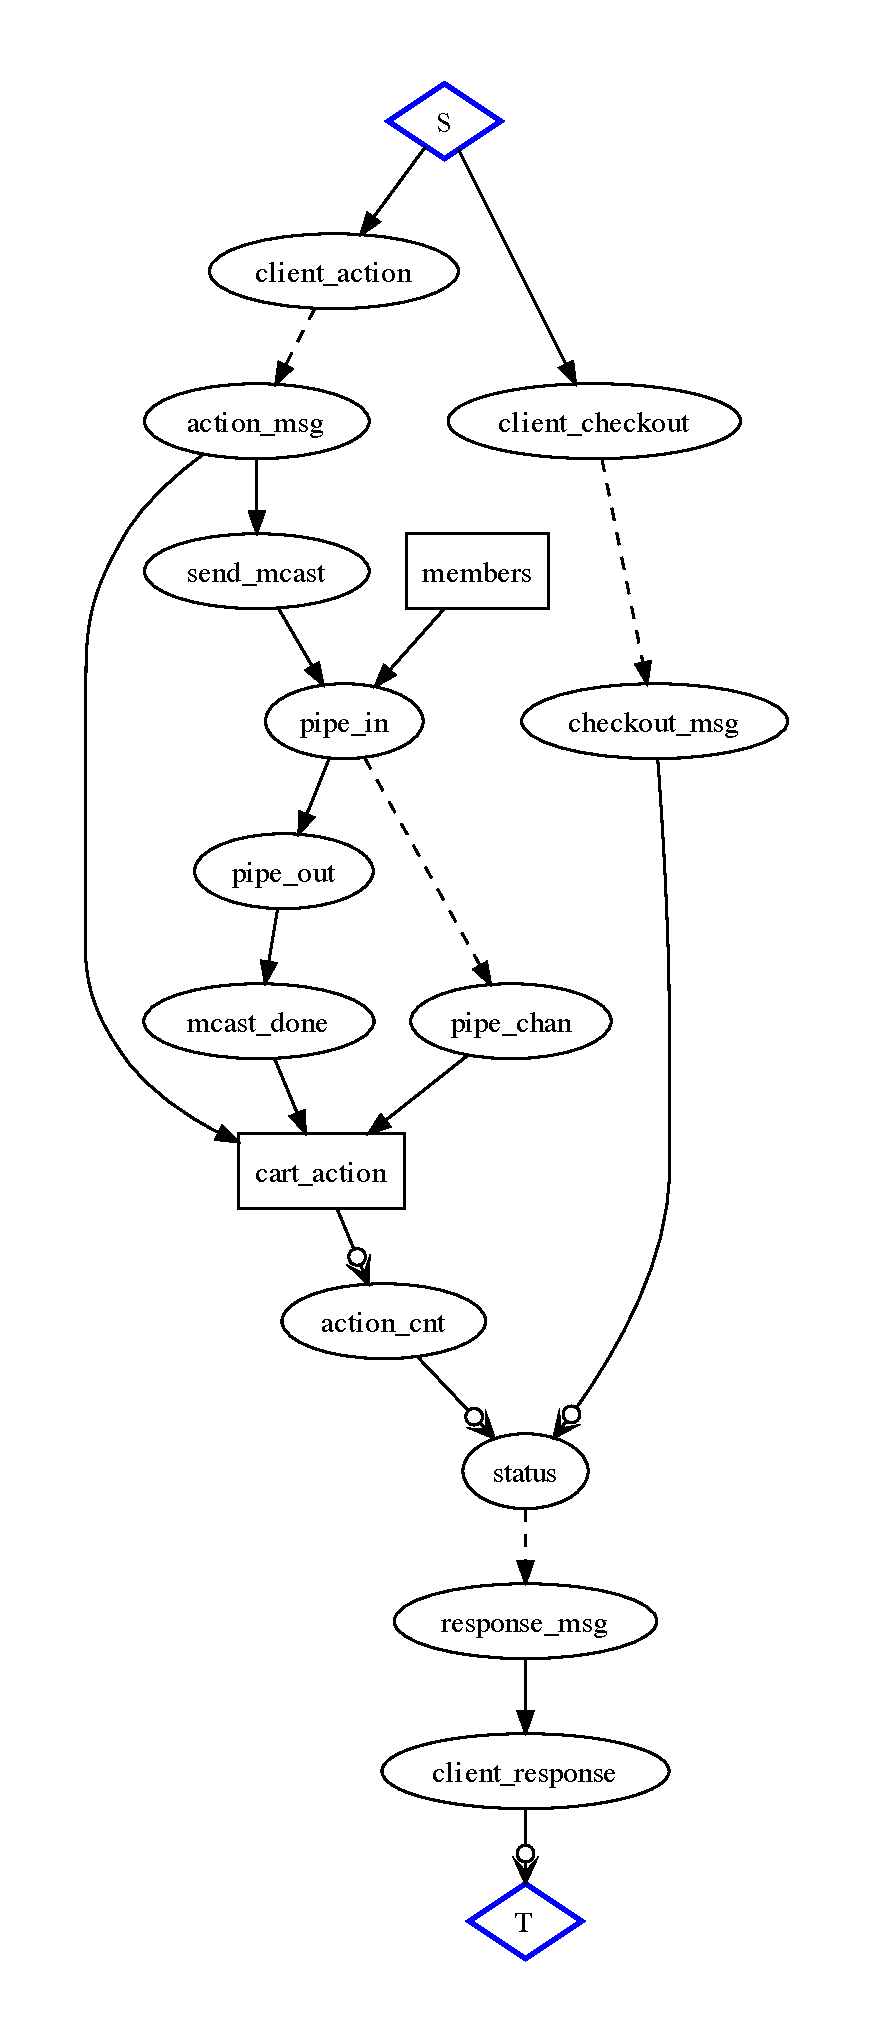
\includegraphics[width=1.2\linewidth]{fig/disorderly_complete.pdf}
\vspace{-10pt}
\caption{Visualization of a fully-specified, replicated disorderly cart program.}
\label{fig:pdg-disorderly-analysis}
\vspace{-2pt}
\end{figure}


%%Intuitively, the ``destructive'' cart based on
%%array mutation should be non-monotonic due to the transience of its state; this should make it sensitive to the order
%%of its inputs.
Figure~\ref{fig:pdg-destructive-kvs-analysis} presents the analysis of the 
``destructive'' shopping cart variant.  Note that
because all dependencies are analyzed, collections defined in the superclass
but not referenced in the code sample
(e.g., \texttt{pipe\_chan}, \texttt{member}) also appear in the graph.
Although there is no syntactic
non-monotonicity in 
Figure~\ref{fig:dest-cart}, the underlying key-value store
uses the non-monotonic \texttt{$<$-} operator to model updateable state.
Thus, while the details of the implementation are encapsulated by the key-value
store's abstract interface, its points of order resurface in the full-program analysis.
Figure~\ref{fig:pdg-destructive-kvs-analysis}
indicates that there are
points of order between \texttt{action\_msg}, \texttt{member} and the temporal cluster,
and between the temporal cluster and itself.
%%This means that the arrival 
%%timing and ordering of both client updates (via \texttt{iaction}) and
%%server replication (via the meta-edge in the temporal cycle from 
%%\texttt{kvput} to itself) may affect the
%%end results.  
This figure also tells the (sad!) story of how we could ensure consistency of the destructive cart implementation: introduce coordination
between client and server---and between the chosen server and all its replicas---for {\em every client action or kvput update}.  
The programmer can easily achieve this coordination by supplying a ``reliable'' implementation
of multicast that awaits acknowledgements from all replicas before reporting completion: this fine-grained coordination is akin to ``eager replication''~\cite{dangers}.  Unfortunately, it would incur the latency of a round of messages per server per client update, decrease system throughput, and make the system fragile in the face of replica failures.

%One coordination technique would require the client to wait for all replicas to
%successfully apply an update before sending a subsequent update.  This would
%involve changing the key-value store to inherit from a reliable delivery
%superclass (implemented in 6 LOC).
%%We can easily achieve coordination without modifying the cart implementation
%%by redefining the key-value store to extend
%%a reliable or quorum-based delivery module instead of the best-effort module
%%that the basic key-value store extends, and require acknowledgement from a server or a %%quorum of servers, respectively.
%%The simplest (and least performant) approach is to require unanimous quorum,
%%approximating ``eager replication''~\cite{dangers} via two-phase commit.
%A programmer could resolve this point of order by adapting the key-value store
%to require reliable delivery to all replicas before acknowledging a client
%update, by making the key-value store inherit from a superclass providing a
%reliable delivery abstraction (6 LOC).
%Such ``eager replication''~\cite{dangers} would incur a cost of a round of
%messages per server per client update, and substantially decrease system
%throughput.  However, it is possible to achieve consistency with far less
%coordination, by writing the shopping cart in a disorderly, rather than
%destructive fashion.
%\wrm{The following is confusing because people might not have this temptation.
%Maybe rephrase to ``a need for synchronization arises, because deletions and
%insertions do not commute''} Because we only care about the set of elements
%contained in the value array and not its order, we might be tempted to argue
%that the shopping cart application is eventually consistent when
%asynchronously updated, and forego the synchronization.  Unfortunately, such
%informal reasoning can hide serious bugs: consider what happens if a delete
%update is received before the addition it was intended to cancel.

% A programmer could resolve this point of order by adapting the key-value store
% to inherit from a reliable delivery superclass (implemented in 6 LOC), requiring 
% acknowledgements from replicas before acknowledging a client update.
% Such ``eager replication''~\cite{dangers} would incur a cost of a round of messages
% per server per client update, and substantially decrease system throughput.  
% \wrm{i don't quite see the point of presenting this straw-man scenario to people.  i think we should just explain that coordination is intuitively needed because deletions don't commute with insertions.}
% \paa{personally I am inclined to keep it.  neil?}
Because we only care about the \emph{set} of elements contained in the value array
and not its order, we might be tempted to argue that 
the shopping cart application is eventually consistent
when asynchronously updated, and forego the coordination logic.  Unfortunately,
such informal reasoning can hide serious bugs. For example, consider what would happen if a delete action for an item arrived at some replica
before any addition of that item: the delete would be ignored, leading to
inconsistencies between replicas.

A happier story emerges from our analysis of the disorderly implementation.
Figure~\ref{fig:pdg-disorderly-base} shows a visualization of the basic
disorderly cart whose implementation is presented in Figure~\ref{fig:dis-cart}.
Its inputs and outputs are channels rather than interfaces, so the dataflow from
source to sink is not completed.  Before we can install the program we must
mixin code that connects input and output interfaces to \texttt{action\_msg},
\texttt{checkout\_msg}, and \texttt{response\_msg}, as the CartClient does
(Figure~\ref{fig:cart-client}).  Note that the disorderly cart has points of
order on all paths, but there are no cycles.

Figure~\ref{fig:pdg-disorderly-analysis} shows the analysis for a complete implementation that mixes in 
both the client code and logic that replicates the \texttt{cart\_action} table via a
best-effort multicast protocol.
Here we see that communication (via \texttt{action\_msg}) between client and
server---and among server replicas---crosses no points of order, so all the
communication related to shopping actions converges to the same final state without coordination.
However, there are points of order upon the appearance of \texttt{checkout\_msg}
messages, which must be joined with an \texttt{action\_cnt} aggregate over the set of updates.  Although the 
accumulation of shopping actions is monotonic, summarization of the cart state
requires us to assume (or rather, prove) that there will be no further cart actions.
%\wrm{i don't think we need to explicitly spell out the race in gruesome detail below.  candidate for cutting.}
%Consider a checkout message and a final update message racing from a client
%to one of the replicas: the order in which they arrive will surely affect
%the contents of the response message.  
The coordination in this graph is much lighter-weight: to
ensure that the response to the client is deterministic and consistently replicated, we need to coordinate once per {\em session} (at checkout), rather than once per shopping action.  This is analogous to the desired behavior in practice~\cite{quicksand}.
% =======
%
% indicates that no points of order are crossed when a client sends an
% \texttt{action\_msg} to a replica, and when replicas exchange
% \texttt{action\_msg} messages during replication.  Thus, all replicas will
% eventually have the same contents in their \texttt{cart\_action} collections,
% even in the absence of coordination.  There is, however, a point of order at
% checkout, when a \texttt{checkout\_msg} message is joined with an aggregate
% over the set of updates.  While the accumulation of \texttt{cart\_action} is
% monotonic, an aggregate cannot be returned until \texttt{cart\_action} is
% complete.
% %requires us to assume (or prove) that there will be no further updates.
% %Consider a checkout message and a final update message racing from a client to
% %one of the replicas: the order in which they arrive will surely affect the
% %contents of the response message.  
% We need only coordinate once per session to ensure that the response to the
% client is deterministic.
% >>>>>>> .r5792

\subsection{Discussion}
Strictly monotonic programs are rare in practice, so adding some amount of
coordination is often required to ensure consistency. In this running example we
studied two candidate implementations of a simple distributed application with
the aid of our language and program analysis. Both programs have points of
order, but the analysis tool helped us reason about their relative coordination
costs.  Deciding that the disorderly approach is ``better'' required us to apply
domain knowledge: checkout is a coarser-grained coordination point than cart
actions and their replication.

By providing the programmer with a set of abstractions that are predominantly
order-independent, Bloom encourages a style of programming that minimizes
coordination requirements. But as we see in the destructive cart program,
it is nonetheless possible to use Bloom to write code in an imperative,
order-sensitive style. Our analysis tools provide assistance in this regard.  Given a
particular implementation with points of order, Bloom's static analysis can help
a developer iteratively refine their program---either to ``push back'' the
points to as late as possible in the dataflow, as we did in this example, or to
``localize'' points of order by moving them to locations in the program's dataflow
where the coordination can be implemented on individual nodes without
communication.
